\documentclass[tikz]{standalone}
\begin{document}
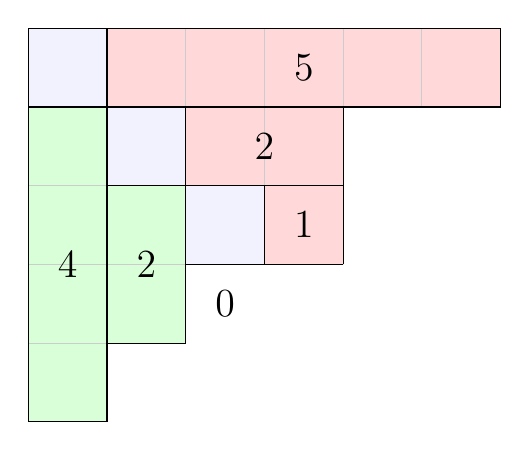
\begin{tikzpicture}
\begin{scope}
  \filldraw[blue!5] (0,0) rectangle (1,-1);\filldraw[blue!5] (1,-1) rectangle (2,-2);\filldraw[blue!5] (2,-2) rectangle (3,-3);
  \filldraw[red!15] (1,0) rectangle (6,-1);\filldraw[red!15] (2,-1) rectangle (4,-2);\filldraw[red!15] (3,-2) rectangle (4,-3);
  \filldraw[green!15] (0,-1) rectangle (1,-5);\filldraw[green!15] (1,-2) rectangle (2,-4);
\end{scope}
\begin{scope}[black!20]
  \draw (0,0) -- (6,0);\draw (0,-1) -- (6,-1);\draw (0,-2) -- (4,-2);\draw (0,-3) -- (4,-3);\draw (0,-4) -- (2,-4);\draw (0,-5) -- (1,-5);\draw (1,0) -- (1,-5);\draw (2,0) -- (2,-4);\draw (3,0) -- (3,-3);\draw (4,0) -- (4,-3);\draw (5,0) -- (5,-1);\draw (6,0) -- (6,-1);\draw (0,0) -- (0,-5);
\end{scope}
\begin{scope}[font=\Large, local bounding box=scope1]  
  \draw (0,0) -- (6,0);\draw (0,0) -- (0,-5);\draw (6,0) -- (6,-1);\draw (0,-1) -- (6,-1);\draw (0,-5) -- (1,-5);\draw (1,0) -- (1,-5);\draw (3.5, -0.5) node{5};\draw (0.5, -3.0) node{4};\draw (4,-1) -- (4,-2);\draw (1,-2) -- (4,-2);\draw (1,-4) -- (2,-4);\draw (2,-1) -- (2,-4);\draw (3.0, -1.5) node{2};\draw (1.5, -3.0) node{2};\draw (4,-2) -- (4,-3);\draw (2,-3) -- (4,-3);\draw (2,-3) -- (3,-3);\draw (3,-2) -- (3,-3);\draw (3.5, -2.5) node{1};\draw (2.5, -3.5) node{0};
\end{scope}
\end{tikzpicture}
\end{document}
